\chapter{Communication}

It is desirable that the system can be controlled from a user interface. The development board supports a OLED display, and two buttons that can be used to interact with the system, but to add more flexibility to the user interface, a GUI is designed on a PC. To data exchange between the DSP and a PC a communication interface is needed. The DSP has an UART hardware device and is chosen to be used as the communication interface. 

\section{Communication between DSP and PC}

As PC's usually do not have a serial port for UART interfacing, a converter is needed.   An USB cable with an integrated FTDI FT232R is used to interface the DSP with a PC as it provides the necessary tools such as automatic instalment of drivers on PC and voltage level conversion between DSP UART and PC USB. The USB cable and FDTI chip are black boxes that are no further explained. The setup of the UART module is described in \autoref{UART_setup}.

The GUI will provide the user accessibility to the necessary tools to control the system. The GUI will have following features:
\begin{itemize}
\item[•]Volume controller
\item[•]Equalizer control
\item[•]System bypass
\item[•]Spectrum analyser
\end{itemize} 

Most of the features are not necessary for the system, but are still nice-to-have for the end user. The volume controller and equalizer are implemented to give the user possibility to change the characteristics of the audio to the users preferences, while the system bypass is implemented to demonstrate the difference between the system and non-processed signal. The spectrum analyser is implemented such that the user can monitor the RMS level of signal if desired. A block diagram of the interface between the PC and DSP is seen in \autoref{fig:communicationBlock}.

\begin{figure}[H]
\centering
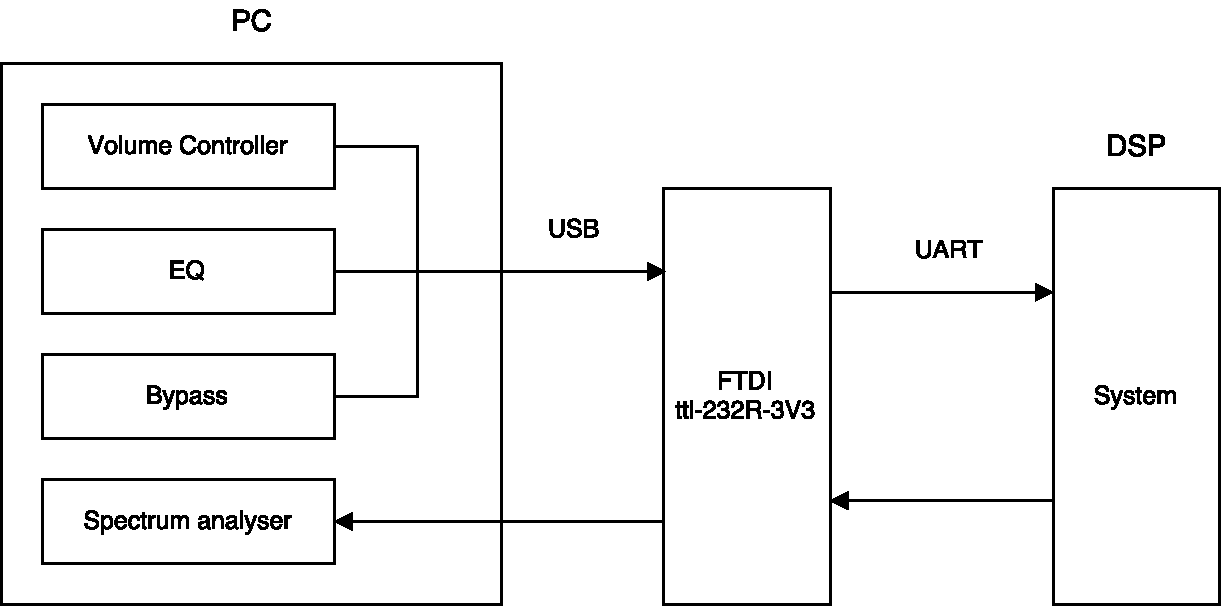
\includegraphics[width=0.75\textwidth]{figures/communicationBlock.pdf}
\caption{Overview of the interface with the DSP.}
\label{fig:communicationBlock}
\end{figure}

Most of the features which will be implemented do not require many design modification, because of the properties the system has. As the spectrum of the audio signal is already divided into octave bands, it is easy equalizer since it only requires a adjustable gain controller to each band and a spectrum analyser only requires an RMS algorithm that can calculate the RMS value of the output of each band. 

A PC program is designed in C\# in Visual Studio as it is easy and straightforward to design GUI's. The final layout and design of the GUI is seen in \autoref{fig:GUI}.

\begin{figure}[H]
\centering
\begin{subfigure}[t]{0.85\textwidth}
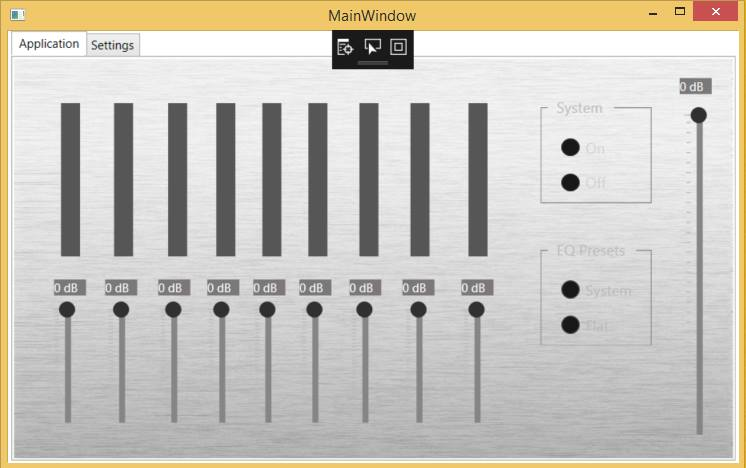
\includegraphics[width=\linewidth]{GUIApp}
	\caption{Control tab for the user.}
	\label{fig:GUIApp}
\end{subfigure}
\hspace{6mm} 
\begin{subfigure}[t]{0.85\textwidth}
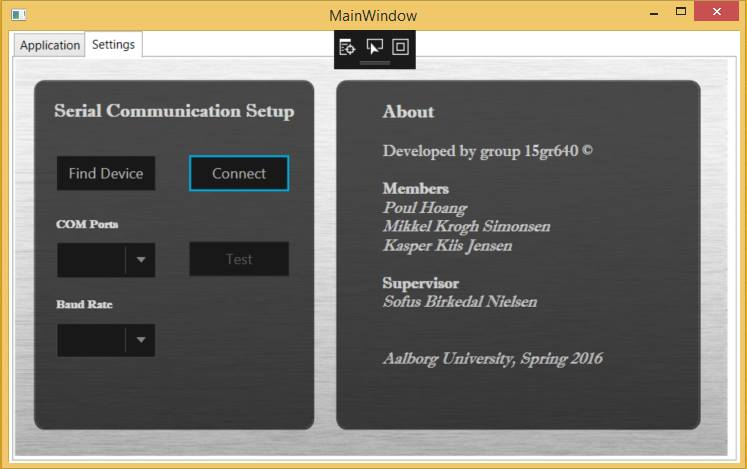
\includegraphics[width=\linewidth]{GUISettings}
	\caption{Communication setup tab.}
	\label{fig:GUISettings}
\end{subfigure}
\caption{Pictures of the GUI.}
\label{fig:GUI}
\end{figure}

There are two tabs available for the user to use. Under settings the user must select the COM port in which the DSP is connected to. After establishing the connection the user can use the user controls in the application tab. From this tab the user can adjust the volume, equalize, bypass the system and observe the RMS value for each band. The next sections will discuss the communication protocol and implementation of each feature.


\section{Volume Controller, Equalizer and Bypass}

The data that is received by the DSP are parameters for the volume controller, equalizer or bypass. In order for the DSP to differentiate between each parameter a communication protocol is needed. The design of the communication protocol can be seen in \autoref{fig:communicationProtocolUART} and consist of a header-byte, a data-byte, and last a check-byte. 
\begin{figure}[H]
\centering
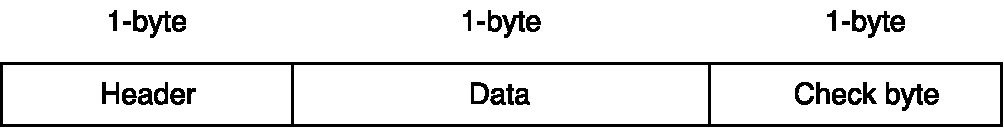
\includegraphics[width=0.75\textwidth]{figures/communicationProtocolUART.pdf}
\caption{Overview of the interface with the DSP.}
\label{fig:communicationProtocolUART}
\end{figure}
The header-byte is used to tell the DSP which parameter the user desires to adjust. If the header byte is 1 then the DSP knows that the incomming data-byte is a equalization gain for the lowest octave band. If the header is 2 then the gain is applied to the second last octave and so on. A header-byte of 10 is a volume control adjustment and 11 is the bypass function. The check-byte is used to ensure that data received is not out-of-sync such that the probability of reading wrong data is lowered.

\subsection*{Volume Controller and Equalizer}
The volume controller is basically just a gain that is applied to the input signal. The resolution of the gain controller is only 7-bit and not 8-bit because of a problem with implementing a 7-bit unsigned char in visual studio. A resolution of 7-bit corresponds to step size of $\frac{1}{128}$. As the steps for the volume controller is implemented in linear scale transmitting 127 corresponds to a gain of 0 dB, 63 to -6 dB, and 0 to $-\inf$. The expression is as follows:
\begin{equation}
G_{\text{dB}} = 20 \log 10 \left( \frac{G}{127} \right)
\end{equation}
The linear solution is as good as a logarithmic volume controller would give a better user experience because of the human hearing, but is easier and sufficient to demonstrate the concept. With the linear scaled volume controller the lowest attenuation before muting the signal is -42.0761 which correspond to transmitting 1. To adjust the gain following code is executed in the DSP.

\begin{lstlisting}[language=C, caption = {Gain adjustment in DSP},label={listingVolume}]
audioIn = (long)audioIn*volume>>7;
\end{lstlisting}

Because the resolution of the volume controller is 8-bit with a signed char (Q7 format), a bit-shifting of 7 must be applied after the multiplication. This is needed as the result of the multiplication is a 23-bit and then quantized to 16-bit.

The implementation of the equalizer is similar to the volume controller. Instead of applying the gain on the input signal the gain is applied on a band-passed signal. The code is seen in \autoref{listingEq}.

\begin{lstlisting}[language=C, caption = {Gain adjustment in DSP},label={listingEq}]
band1 = (long)array[184]*gainBand1>>7;
\end{lstlisting}

The resolution of the equalizer is the same as the volume controller. 

\subsection*{Bypass}
The simplest type of bypass is by setting the input signal of the audio codec as the output. Since the the audio signal in the system is delayed, changing the output between bypass and system will give and unpleasant transition. In order to give a smoother transition, a delay must be applied to the bypassed input signal as well. The total amount of delay must the same delay applied to stage 1 in the multistage system. The total amount of delay in stage one is calculated to 5333 sample delay. The delay corresponds to 111 ms for a 48 kHz system. The implementation of the delay is seen in \autoref{listingByPass}.

\begin{lstlisting}[language=C, caption = {Delay function for bypass},label={listingByPass}]
int16 delayBypass(int16 dataIn, int16 *dataBuffer, int16 *dataPtr){
	int16 temp;
	temp = dataBuffer[*dataPtr]; // Store oldest data in temp
	dataBuffer[*dataPtr] = dataIn;	// Overwrite with newest data
	(*dataPtr)++;	// Increment data pointer
	if (*dataPtr == 5333){	
		*dataPtr = 0;	
	}
	return temp;
}
\end{lstlisting}

Before overwriting the oldest data in the data buffer, the oldest data is stored the a temporary variable. Afterwards the new data is overwriting the oldest data. The oldest data in the temporary variable is then returned.

As the delay is large the delayed samples are stored in Single Access RAM (SARAM) block 2. To do so the pragma directive is used to tell the compiler that it is desired that the data for the delay is stored in SARAM.

\begin{lstlisting}[language=C, caption = {Pragma for delay buffer for bypass.},label={listingPragma}]
#pragma DATA_SECTION(BypassBuffer, ".BypassArray")
int16 BypassBuffer[5333];
\end{lstlisting}


\section{Spectrum Analyser}

To implement a spectrum analyser RMS-calculators are implemented as a C-function for all bands in the system. There are multiple octave bands in the system and to differentiate between each band another communication protocol is implemented. The implemented communication protocol is seen in \autoref{fig:communicationProtocolUARTTransmit}.

\begin{figure}[H]
\centering
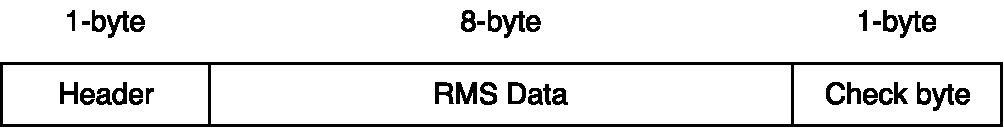
\includegraphics[width=0.75\textwidth]{figures/communicationProtocolUARTTransmit.pdf}
\caption{Overview of the interface with the DSP.}
\label{fig:communicationProtocolUARTTransmit}
\end{figure}

The communication protocol consist of a header-byte and 8 data byte and a check byte in the end to reduce the amount of error readings. The cheack-byte has the same value as the header byte. The first byte in "RMS data" is the RMS value for the lowest octave band while the last is the highest.

The RMS-function is called after the RMS compression. The C-function for the RMS-function is seen in \autoref{listingRMSuart}

\begin{lstlisting}[language=C, caption = {Calculate RMS value},label={listingRMSuart}]
uint8 RMScalculate(int16 *dataBuffer, int16 dataIn, int16 *BufferPtr, long *sum){
	// Initialize local variables
	uint8 result; long temp;
	
	// Calculate RMS^2
	*sum = *sum - dataBuffer[*BufferPtr]; // Substract the oldest data from sum
	temp = (long)dataIn*dataIn;	// Square the new sample
	dataBuffer[*BufferPtr] = temp>>15;	// Bit-shift and store in data buffer
	*sum = *sum + dataBuffer[*BufferPtr];
	result = ((*sum)>>4)>>5;				// Calculate new RMS^2
	
	// Increment data pointer
	(*BufferPtr)++;
	if (*BufferPtr == 16){ 
		*BufferPtr = 0;
	}
	
	return result;
}
\end{lstlisting}
\todo[inline]{Fejl i koden! BufferPtr skal sammenlignes med 32 og ikke 16! Samt bit shift på 10 og ikke 9.}

The RMS function is essentially the same to the RMS algorithm described under the compressor section. The function calculates the RMS$^2$ and transmits that value to the GUI which handles the square root function.

% Appendix - Baudrate, register setup. Husk external bus setup.

